\begin{figure}[ht]
 	\centering
	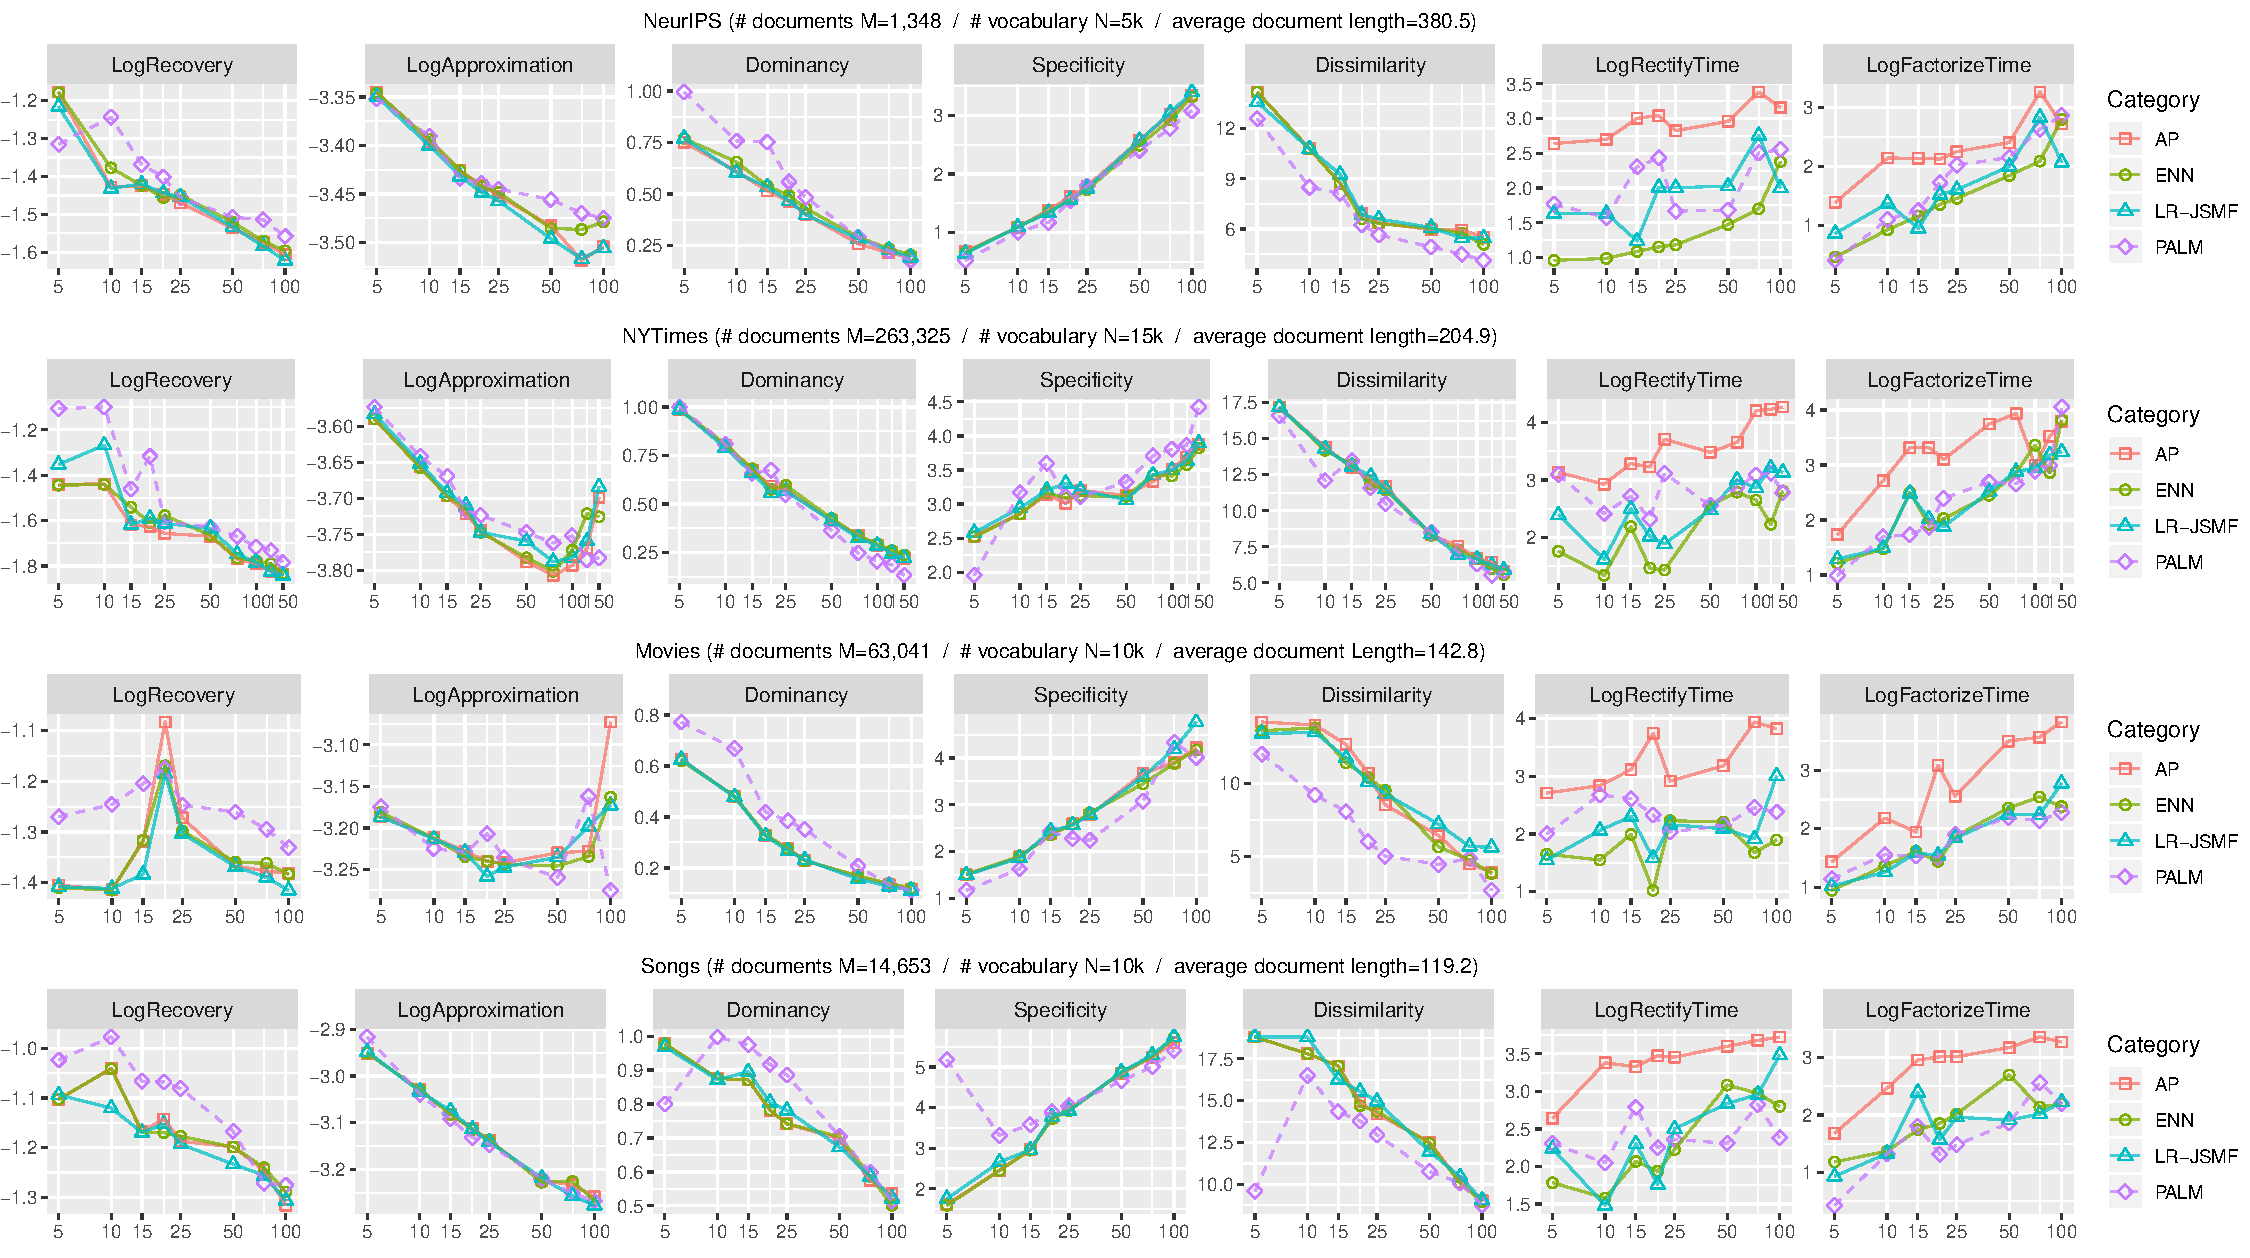
\includegraphics[width=0.97\textwidth, trim={1.0cm 1.0cm 1.0cm 0.0cm}]
	{./ch4/pics/real_MethodsPerTopics_new-plain.pdf}
	\caption{Experiment on four datasets. ENN and LR-JSMF mostly agree with AP,
	whereas PALM has slight inconsistency. The general information of each dataset
	is above the corresponding row. Recovery, approximation, and runtimes are in
	$\log_{10}$ scale. Note that ENN and LR-JSMF are almost two orders of
	magnitude faster than AP. The $x$-axis indicates the number of clusters $K$.
	Lower numbers in $y$-axis are better except Specificity and Dissimilarity.} 
	\label{fig:results-topics}
\end{figure}

A good factorization should be accurate, meaningful, and fast.
In two series of experiments, we show that LR-JSMF maintains model quality while
running in a fraction of the space and time needed for the original JSMF method.
Previous methods have required truncation of the vocabulary even to run on
consumer-grade computers. We show not only that we are able to handle
increasingly large vocabularies without loss of speed, but that using larger
vocabularies measurably improves model quality relative to truncated vocabularies.

For the first series of experiments, we measure the accuracy of each
rectification component as well as the entire pipeline of LR-JSMF. To produce a
strong baseline, we begin with constructing the full co-occurrence $\BC$ from
each of our datasets $\BH$ by \eqref{eqn:unbiased}, and produce the rectified
$\BC_{AP}$ by running Alternating Projection (AP) on $\BC$. Next we compress
$\BC$ into $\BY_{ENN}$ and $\BY_{PALM}$ by running ENN (50 iterations, $|I|\Eq
10K \Plus 1000$) and PALM (100 iterations, $s\Eq1e^{-4}$). For testing our
complete low-rank pipeline, we also construct $(\BV, \BD)$ directly from the raw
data $\BH$ by the randomized eigen-decomposition in Algorithm \ref{alg:lr-jsmf},
learning the compressed statistics \smash{$\BY_{LR-JSMF}$} again by running ENN
initialized with \smash{$\BV \sqrt{\BD}$}. Then we run the Anchor Word algorithm
(AW) on $\BC_{AP}$ and the Low-rank Anchor Word algorithm (LAW) on each of $\BY_
{ENN}$, $\BY_{PALM}$, and $\BY_{LR-JSMF}$.

The goal of rectification is to apply spectral inference to data that does not
follow our modeling assumptions, so we evaluate on real data. In addition to two
standard datasets from the UCI Machine Learning repository (NeurIPS papers and
New York Times articles), we also use two non-textual datasets (Movies and
Songs) previously used to demonstrate the performance of full algorithm with
AP-rectification in \cite{moontae2015nips}. Although our ultimate goal is to
extend JSMF to large vocabularies, we use the same restricted vocabulary as 
\cite{moontae2015nips} for a fair comparison in the first series of experiment.

Figure \ref{fig:results-topics} shows the overall performance of the learned
topic clusters from these four datasets with increasing number of clusters $K$.
Low \textbf{Recovery} error $\frac{1}{N}\sum_i\|\BCbar_{i\ast} - \BBreve_{i\ast}
\BCbar_{S\ast}\|_2$ implies that the learned anchor objects successfully
reconstruct the co\hyp{}occurrence space of the entire objects. Low 
\textbf{Approximation} error $\|\BC-\BB\BA\BB^T\|_2$ means that our
factorization captures most of information given in the unbiased co
\hyp{}occurrence statistics. In real data, low \textbf{Dominancy} $\frac{1}
{K}\sum_k \BA_{kk}$ implies that our models learn more correlations between
clusters. High \textbf{Specificity} \smash{$\frac{1}{K} \sum_k \text{KL}(\BB_
{\ast k}||\sum_i\BC_{\ast i})$} indicates that the learned clusters are
different enough from the corpus distribution, whereas high 
\textbf{Dissimilarity} counts the average number of objects in each cluster that
do not occur among top $20$ in other clusters, showing the interpretable
difference across the learned clusters. We do not report the Cluster Coherence
because it often measures deceptively \cite{chang2009reading}. The first five
columns show that ENN and LR\hyp{}JSMF learn approximately same clusters as JSMF
with the full AP, showing no visible loss in accuracy across all settings. More
importantly, the randomness we introduced into LR\hyp{}JSMF results in a very
low variance over a number of runs. This is important as the stability of
spectral inference is a major advantage relative to MCMC or Variational
Inference. Although PALM deviates a small amount from the other three methods in
a few cases, it mostly achieves the same level of accuracy and follows the
overall trend closely. In terms of runtimes, all of our methods have clear
advantage over AP, gaining $1\sim2$ orders of magnitude speedup in most
situations. Even for applications on relatively small vocabulary sizes, our
algorithms shows a notable improvement in efficiency.

\begin{figure}[ht]
 	\centering
	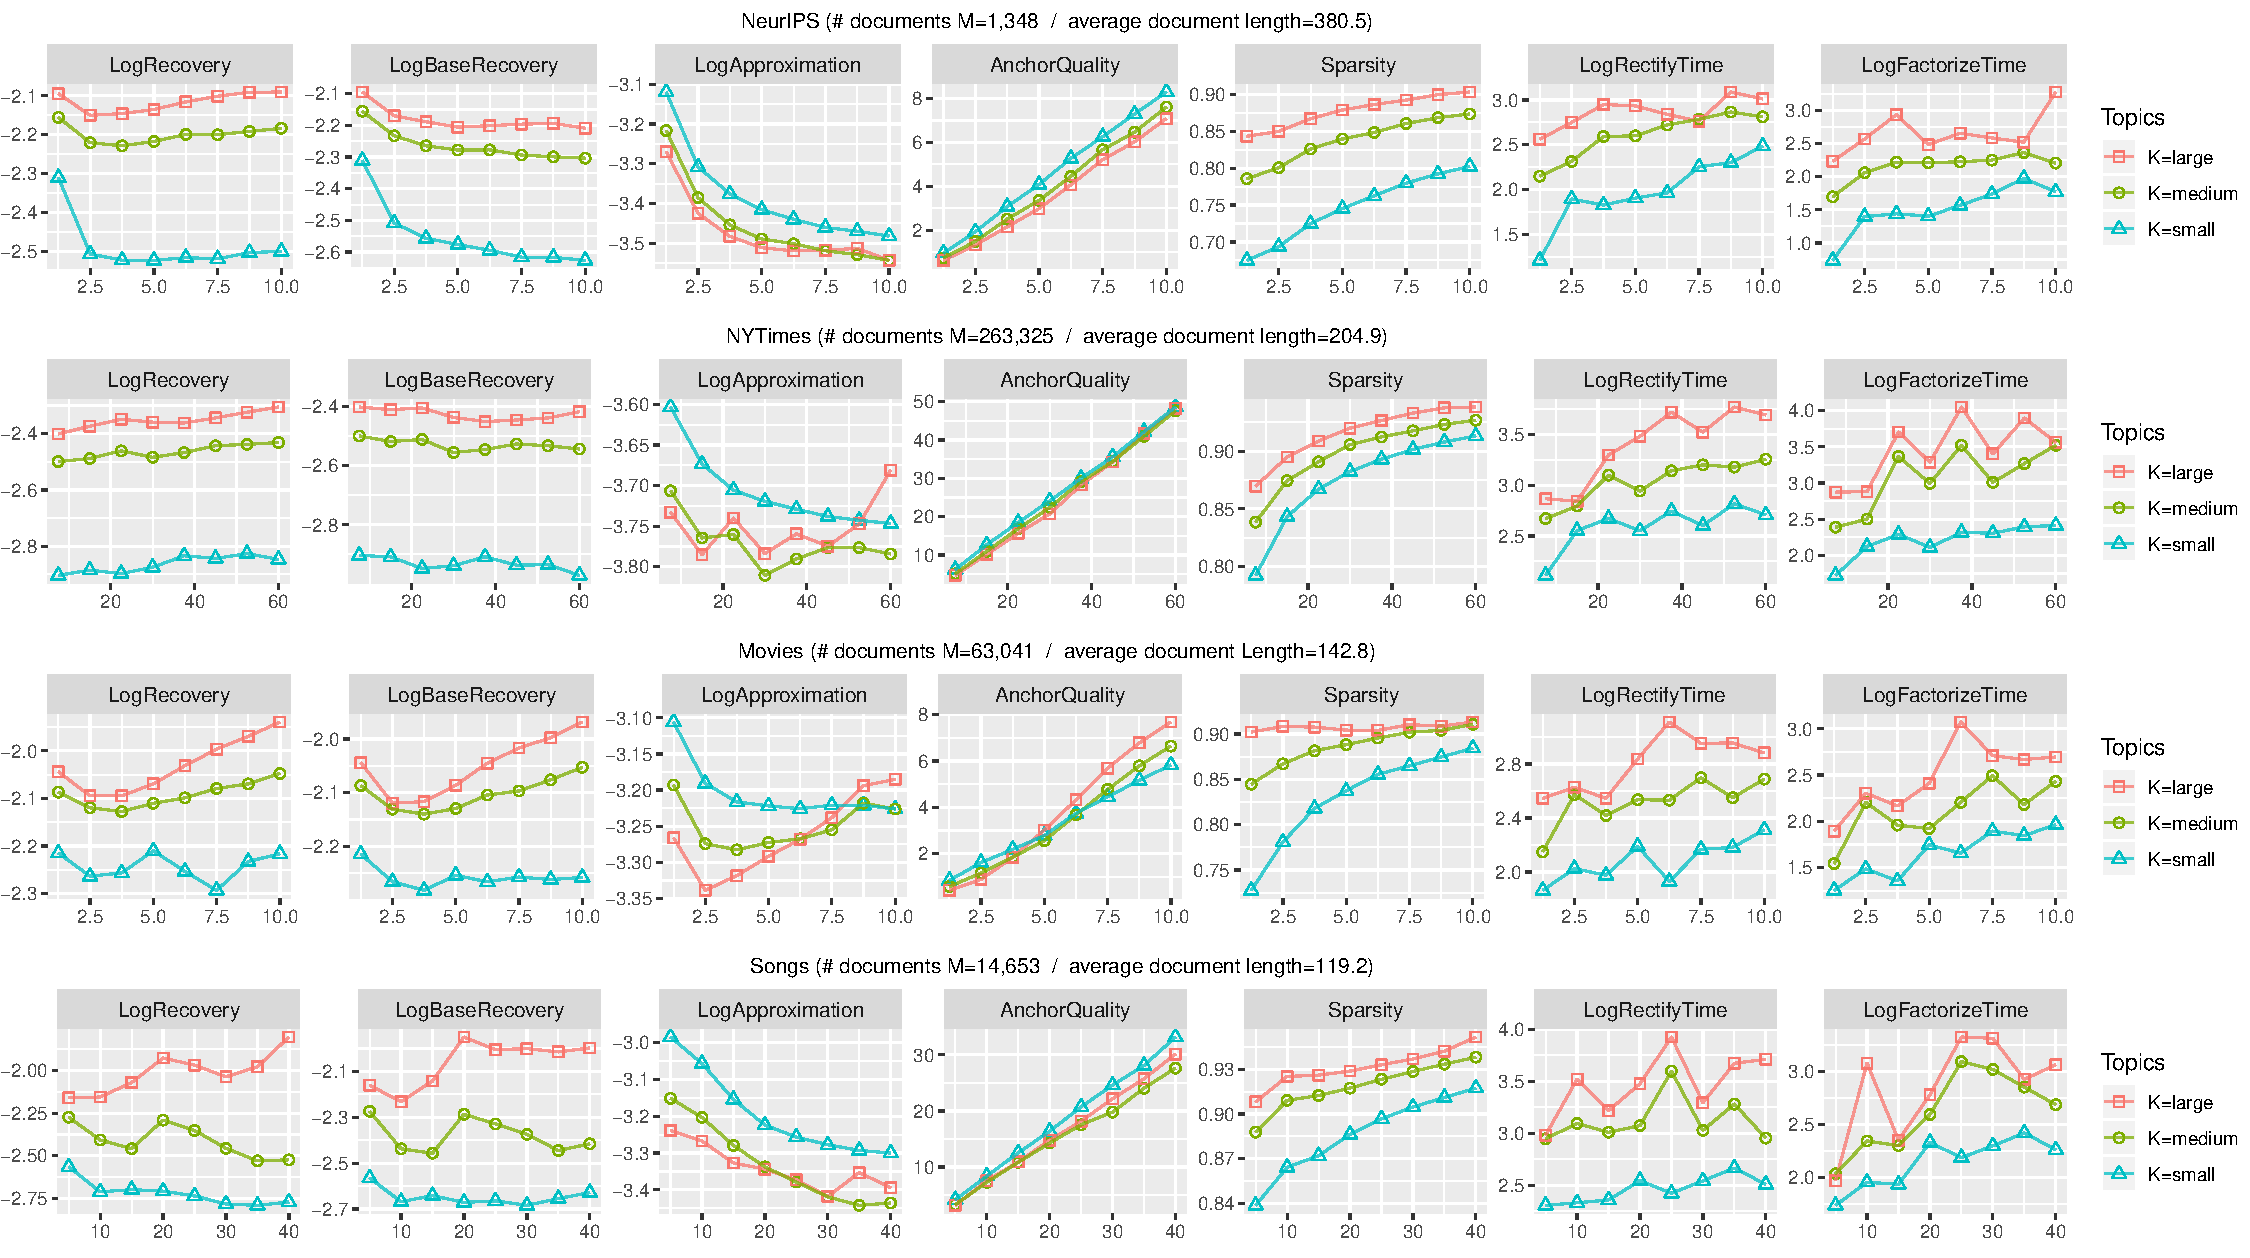
\includegraphics[width=0.97\textwidth, trim={1.0cm 1.0cm 1.0cm 0.0cm}]
	{./ch4/pics/real_TopicsPerVocabs_new-plain.pdf}
	\caption{As we increase the vocabulary size for four collections, anchor
	quality and sparsity improve, but running time is stable. The $x$-axis
	indicates the vocabulary size $N$ in thousands. Values above 15k will not fit
	in memory on standard hardware with previous algorithms.}
	\label{fig:results-vocabs}
\end{figure}

For the second series of experiments, 
we create eight corpora $\{\BH_N, \BH_{2N}, ..., \BH_{8N}\}$ for each dataset
$\BH$ by tailoring their vocabulary sizes as multiples of a base vocabulary of
$N$ objects. In this case we are not able to compare LR-JSMF to previous methods
because we cannot store the full co\hyp{}occurrence matrices for the larger
vocabulary: these models would be impossible. Figure \ref{fig:results-vocabs}
illustrates the overall performance of the learned small/medium/large size
clusters with increasing vocabulary size $N$. Low \textbf{BaseRecovery} means
that the anchor objects from the models with larger vocabulary better
reconstruct the objects in our base vocabulary ($\BH_N$). High  
\textbf{AnchorQuality} indicates that the average rank of the anchor objects
$s_k$ in every other topic clusters than $k$ is high, implying the anchor
objects rarely contribute to other clusters than their own. High 
\textbf{Sparsity} \smash{$(\frac{1}{K} \sum_k \frac{\sqrt{N} - (\|\Bb_k\|_1 /
\|\Bb_k\|_2)}{\sqrt{N} - 1})$} \cite{Hoyer2004} says that our topic clusters are more concentrated on specific objects.

We observe the quality of anchors increases with increasing vocabulary size,
verifying that using larger vocabularies helps better satisfy the separability
assumption. We also verify that a large vocabulary often better approximates the
co\hyp{}occurrence statistics and better reconstructs the co\hyp{}occurrence
space of the \textit{base} vocabulary, but these patterns are not always
consistent in non-textual datasets. In contrast, Sparsity consistently improves,
increasing the interpretability of the learned clusters. Most excitingly, the
running times of ENN and LAW show the scalability of our new rectification and
low-rank algorithm, thereby demonstrating that LR-JSMF is an efficient and
robust pipeline.

Finally, we have also inspected the qualitative behavior of the recovered
clusters, as we increase the vocabulary size. The topic clusters become
significantly more specific, while the clustering of objects is more
conspicuous. Figure \ref{fig:top_words} shows how using a larger vocabulary size
can lead to more distinguishable topics, especially as it allows us to make use
of words that are relatively rare, but used in much narrower contexts. Going
from left to right, we can observe that the set of topic words become more and
more specific: for instance, the topic corresponding to the third row is
slightly vague when observing just the left half of the row, while as we
increase the vocabulary size beyond 5000, we gain access to highly
topic-specific words such as hjb (Hamilton-Jacobi-Bellman equation) or pid 
(Proportional Integral Derivative), which signifies the row's pertinence to
dynamical and control systems. The flip side of the figure shows that words we
would normally consider as non-topical can often be assigned high contributions
towards certain topics. The strong red shade on the bottom left indicates that
words such as ``equivalent'' or ``cambridge'' are strongly connected to the
machine learning literature.

\begin{figure}[ht]
 	\centering
	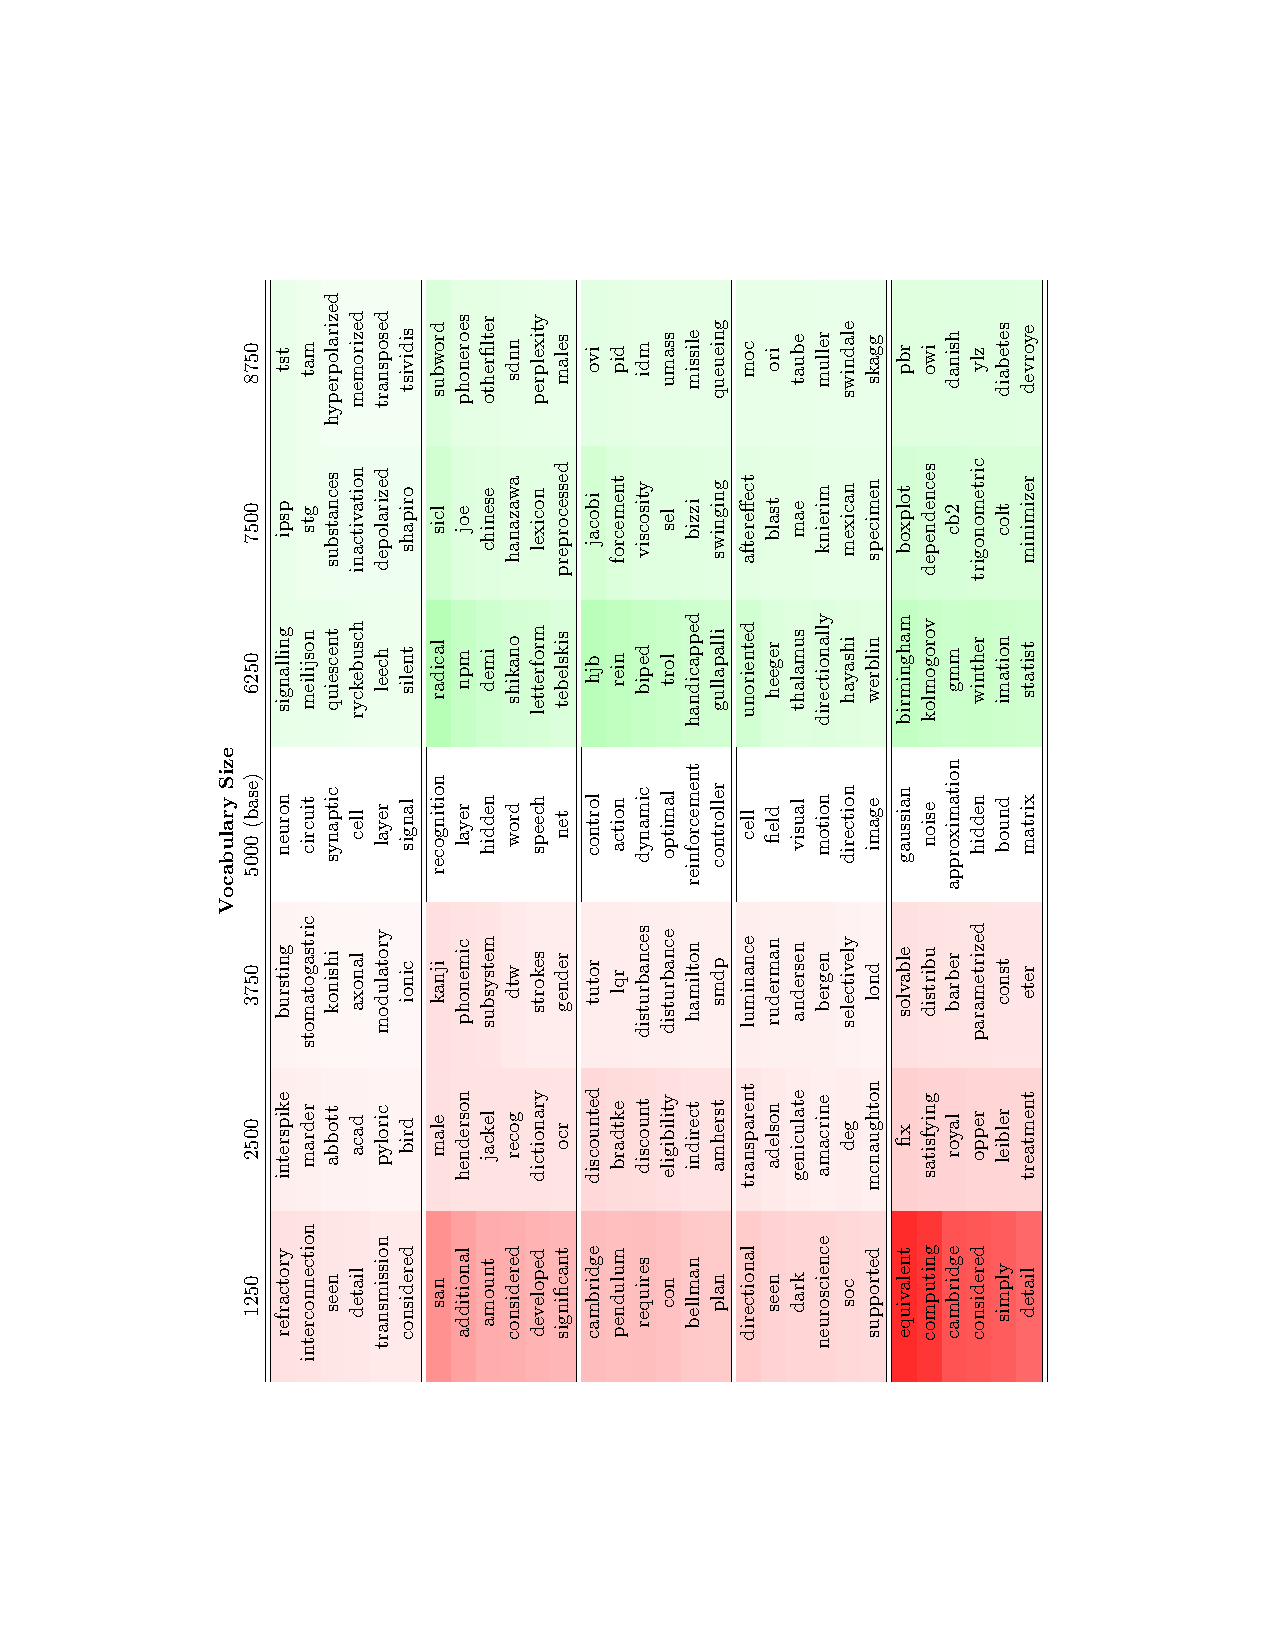
\includegraphics[angle=270, width=1.0\textwidth, trim={2.0cm, 4.5cm, 2.0cm,
	4.5cm}]{./ch4/pics/topWordsFull.pdf}
	\vspace*{-40px}
	\caption{Losses or gains in topic words depending on the vocabulary size. Each
	row represents a topic from the NeurIPS dataset, with the top 6 topical words
	shown in the middle column. The red and green cells denote topic words that
	are lost or gained by shifting the vocabulary size from the default size 5000,
	respectively. The intensities of the colors indicate the words' contributions
	towards the specific topic.} 
	\label{fig:top_words}		
\end{figure}